\subsection{Briefing avec Leon Turrou}

\paragraph{}

\begin{wrapfigure}{r}{50mm}
\begin{center}
 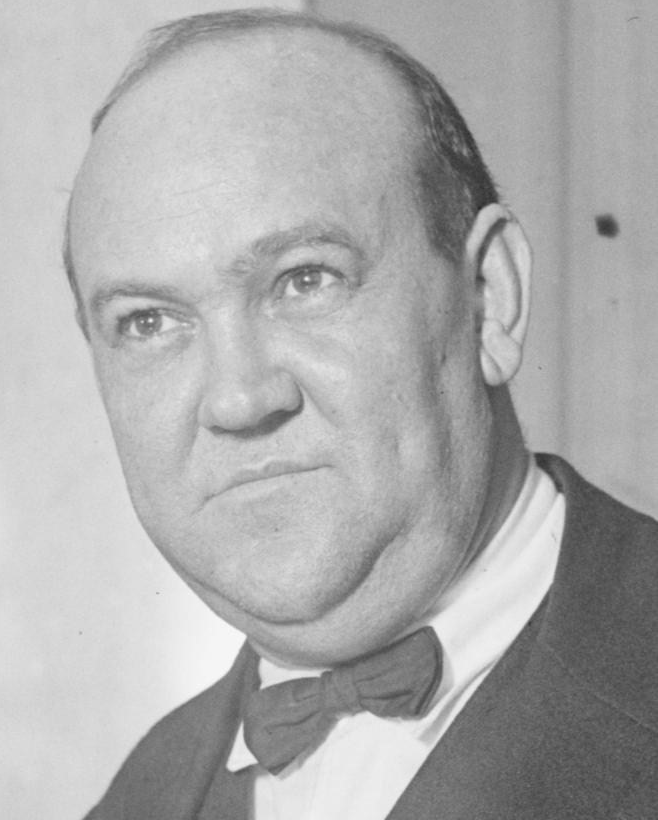
\includegraphics[width=40mm]{../pnjs/gaston-means-1924.png}
\end{center}
\caption{Gaston Means - 1924}
\end{wrapfigure}

\paragraph{} PJs envoyés arrêtent \gls{gms} suite à la plainte \gls{ewm}, mais ce dernier en profite pour faire le malin 
auprès d'eux, prétendant en savoir bcp sur l'affaire : \emph{Sans moi, vous pouvez déjà oublier tout espoir de retrouver le 
bébé en vie}. Ils l'arrêtent le matin à Washingthon, à son domicile, et se rendent ensuite dans le bureau de \gls{ejh}, 
\emph{le siège du gouvernement}.

\begin{wrapfigure}{l}{60mm}
\ovalbox{
  \scalebox{0.9}{
  \begin{minipage}{2in}
  \textbf{Et si les investigateurs n'assistent pas à l'échange ?}
  \begin{center}------\end{center}
  \paragraph{} Dans ce cas, le cadavre de la jeune femme, qui n'aurait pas survécu à la noyade
  malgré le sort du Profond, réapparaitra le lendemain, non loin de là. Comme les agents auront très probablement rapporté leur escapades dans le
  Bronx à \gls{ejh}, ce dernier ne manquera pas de faire le lien - ses assistants ont reçu ordre, juste après le rapport des investigateurs de lui 
  signaler tout rapport ou évènement étranges à New York et dans les environs. Néanmoins, l'information ne parviendra pas exactement au \gls{fbiHq},
  et les investigateurs n'auront vent de ceci que la nuit d'après, soit le 3 mai.
  \end{minipage}
  }
}
\end{wrapfigure}

\paragraph{} \gls{ejh} sort \gls{lgt} de l'opération car il est connu comme le loup blanc par les différents intervenants et 
qu'il le soupçonne, probablement à raison, de manquer de la subtilité nécessaire pour une telle opération. (PJs rapportent à 
\gls{ejh} à midi qui les informe du rdv secret de ce soir entre \gls{jafsie} et les kidnappeurs.

% \todo{ décrire le contexte d'un tel rendez vous, la mise en scène de \gls{ejh}, donner des conseils sur l'interprétation et la
% pression lié à un tel rendez vous. Emphase de \gls{ejh} }